\chapter{Fluid Instabities}
\label{cha:fluid-instabities}
\label{sec:instabilities}
\index{fluid mechanics!instabilities}
\section{Gravity Waves and Rayleigh-Taylor Instability}
\label{sec:gravitywaves}
\index{fluid mechanics!gravity waves}
\index{gravity waves}
\index{Rayleigh-Taylor instability}
\index{fluid mechanics!instabilities!Rayleigh-Taylor}

\begin{figure}
\begin{center}
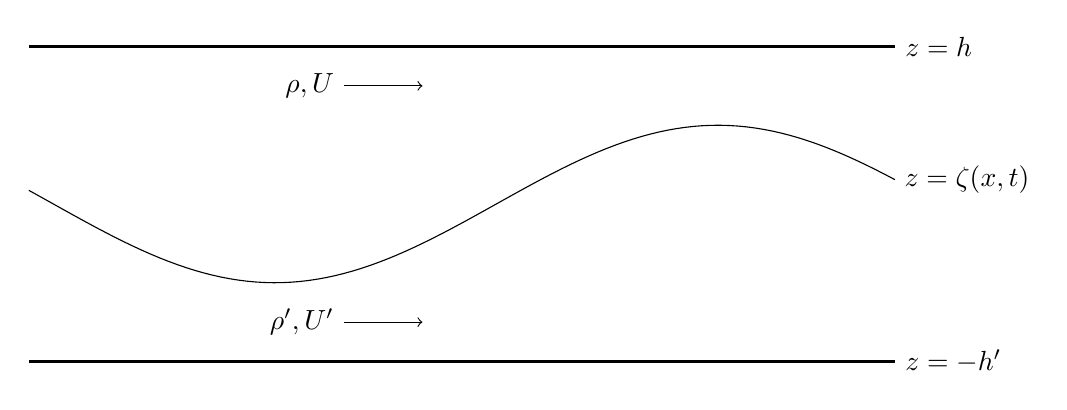
\begin{tikzpicture}
\draw [thick] (0,2) -- (11,2) node [right] {$z=h$} (0,-2) -- (11, -2)
node [right] {$z=-h'$} ;
\draw plot [domain=0:11,samples=100] ( \x, {sin(32*\x+170)}) node [right] {$z=\zeta(x,t)$} ;
\draw [<-] (5,1.5) -- (4,1.5) node [left] {$\rho, U$} ; 
\draw [<-] (5,-1.5) -- (4,-1.5) node [left] {$\rho', U'$} ; 
\end{tikzpicture}
\end{center}
\caption{Shearing flow in a stratified fluid}
\end{figure}
Let's imagine a different type of wave on a fluid.  Let's imagine we
have two fluids in a gravitational field.  The lower fluid has density
$\rho'$, velocity $U'$ and thickness $h'$ and the upper fluid has
density $\rho$, velocity $U$ and
thickness $h$.  Let's have $\zeta(x,t)$ denote the displacement of the
interface in the $z-$direction.  Let's assume that both fluids are
incompressible and the flow is irrotational, so we can define
\begin{equation}
{\bf v} = -\nabla \Phi ~\mathrm{and}~ {\bf v}' = -\nabla \Phi'
\end{equation}
where
\begin{equation}
\Phi = -U x + \phi~\mathrm{and}~ \Phi' = -U' x + \phi'.
\end{equation}
To make further progress let us assume that the displacement of the
interface has the form
\begin{equation}
\zeta(x,t) = A \cos \left ( k x - \omega t \right )
\end{equation}
and furthermore let velocity potentials also have a similar dependence
\begin{equation}
  \phi = C \sin \left (k x - \omega t\right ) f(z)~\mathrm{and}~
  \phi' = C' \sin \left (k x - \omega t\right ) f'(z).
\end{equation}
Because the fluids are assumed to be incompressible, we have $\nabla^2
\phi=0$ and the boundary condition gives $\partial \phi/\partial z=0$
at $z=h$ and similarly for lower fluid, so we have 
\begin{eqnarray}
\phi &=& C \sin \left (k x - \omega t\right ) \cosh \left [ k(z-h)
\right ] \\
\phi' &=& C' \sin \left (k x - \omega t\right ) \cosh \left [ k(z+h')
\right ]. 
\end{eqnarray}
The Lagrangian derivative of the displacement of the interface
$D \zeta(x,t)/Dt$ gives the vertical velocity of the fluid at the
interface, so
\begin{equation}
-\pp{\phi}{z} = \pp{\zeta}{t} + U \pp{\zeta}{x}~\mathrm{and}~
-\pp{\phi'}{z} = \pp{\zeta}{t} + U' \pp{\zeta}{x}.
\end{equation}
This yields a relationship between the constants $A$, $C$ and $C'$,
the wavenumber and frequency,
\begin{eqnarray}
A \left ( k U - \omega \right ) &=& - k C \sinh k h, 
\label{eq:868}
\\
A \left ( k U' - \omega \right ) &=&  k C' \sinh k h'.
\label{eq:869}
\end{eqnarray}
We seek a relationship between $\omega$ and $k$, so we require an
additional equation to eliminate the unknowns $A$, $C$ and $C'$.
Specifically, the pressure on each side of the interface must be
equal.  To examine the pressure let's look at Euler's equation
for the ideal fluid (Eq.~\ref{eq:631}) and substitute ${\bf V}=-\nabla
\Phi$ to yield
\begin{equation}
-\pp{\nabla \Phi}{t} + \frac{1}{2} \nabla V^2 = -\frac{\nabla P}{\rho}
- g {\hat z}.
\end{equation}
Since the fluid is incompressible we can write
\begin{equation}
\nabla \left [ -\pp{\Phi}{t} + \frac{V^2}{2} + \frac{P}{\rho} + g h
\right ] = 0,
\end{equation}
so for each fluid we have
\begin{eqnarray}
-\rho \pp{\Phi}{t} + \rho \frac{v^2}{2} + g z \rho + p &=& B(t), \\
-\rho \pp{\Phi'}{t} + \rho' \frac{v'^2}{2} + g \rho' z + p &=& B'(t).
\end{eqnarray}
At the upper and lower surface the velocity of the perturbation
vanishes and $p(z=-h')-p(z=h)$ must equal $g \rho h + g \rho' h'$, so
\begin{equation}
B(t) - B'(t) = \frac{\rho U^2}{2} - \frac{\rho' U'^2}{2}.
\end{equation} 
Let's take the difference of the two Bernoulli equations and evaluate
it at $z=\zeta(x,t)$ to yield
\begin{equation}
\rho \left ( -\pp{\phi}{t} - U \pp{\phi}{x} + g \zeta \right )=
\rho' \left ( -\pp{\phi'}{t} - U' \pp{\phi'}{x} + g \zeta \right ).
\end{equation}
to first order in the small quantities $\phi$ and $\phi'$.
Substituting the expressions for $\phi$, $\phi'$ and $\zeta$ yields
\begin{equation}
\rho \left [ C \cosh kh \left ( \omega - k U \right ) + g A \right ] = 
\rho' \left [ C' \cosh kh' \left ( \omega - k U' \right ) + g A \right ] .
\end{equation}
Combining this result with Eq.~\ref{eq:868} and~\ref{eq:869} yields
the equation,
\begin{equation}
\rho \left ( \omega - k U \right )^2 \coth kh  +
\rho' \left ( \omega - k U' \right )^2 \coth kh' = k g \left (\rho' -
  \rho \right ),
\end{equation}
and the dispersion relation,
\begin{eqnarray}
\frac{\omega}{k} &=& \frac{\rho U \coth kh + \rho' U'\coth k h'}{\rho
  \coth kh + \rho' \coth k h'} \pm \nonumber \\
& &~~~ \left [ \frac{g}{k} \frac{\rho' - \rho}{\rho
  \coth kh + \rho' \coth k h'} - \frac{\rho \rho' \coth kh \coth kh' \left ( U - U' \right )^2}{\left (\rho
  \coth kh + \rho' \coth k h' \right)^2 } \right ]^{1/2}.
\label{eq:870}
\end{eqnarray}
The first interesting limit is where $U=U'=0$ which yields the simpler expression
\begin{equation}
\frac{\omega^2}{k^2} =  \frac{g}{k} \frac{\rho' - \rho}{\rho \coth k h +
    \rho' \coth k h'} 
\label{eq:769}
\end{equation}
If $\rho' > \rho$, then $\omega^2>0$ and we have a stable wave.  There
are several interesting limits to this result.
\begin{itemize}
\item If $\rho=0$, then $\omega^2 = g k \tanh kh$.
\item If $\rho=0$ and $kh \gg 1$, then $\omega^2 = g k$ (deep-water waves).
\item If $\rho=0$ and $kh \ll 1$, then $\omega^2 = g h k^2$ (shallow-water
  waves).
\item If $\rho\neq 0$, $kh' \gg 1$ and $kh \gg 1$, then (both liquids
  very deep)
\begin{equation}
\omega^2 = \frac{kg (\rho' - \rho)}{\rho+\rho'}
\label{eq:770}
\end{equation}
\item If $\rho\neq 0$, $kh' \ll 1$ and $kh \ll 1$, then (long waves)
\begin{equation}
\omega^2 = k^2 \frac{g (\rho' - \rho) h h'}{\rho h'+\rho' h}
\label{eq:771}
\end{equation}
\end{itemize}

On the other hand if $\rho' < \rho$, then $\omega^2 < 0$ and the
perturbation simply grows (it does not oscillate).  This is the
Rayleigh-Taylor instability.  This instability occurs whenever a low
density gas underlies a higher density gas, for example in a supernova
explosion.  The gravitational acceleration $g$ can be due to gravity
(as in a supernova) or due to a deceleration of the fluid, if a
low-density fluid plows into a high-density fluid.  According to
Eq.~\ref{eq:771} the smallest scales have the highest growth rates.
This is countered by viscosity and surface tension, so a
particular scale dominates the growth at least initially.

\section{Kelvin-Helmholtz or Shearing Instability}
\label{sec:kelvin-helmholtz-or}
\index{Kelvin-Helmholtz instability}
\index{shearing instability}
\index{fluid mechanics!instabilities!shearing}

If we look at the term in the brackets in Eq.~\ref{eq:870} for $U \neq
U'$ we see that if $g=0$ waves with all values of $k$ are unstable and if $g\neq
0$ for sufficiently large values of $k$ (small wavelengths), waves are
unstable even if $\rho'>\rho$.  The critical value of $k$ is
\begin{equation}
k_\mathrm{crit} = \frac{g}{\left (U - U'\right)^2} \frac{\rho'-\rho}{\rho \rho' } \frac{\rho
  \coth kh + \rho' \coth k h'}{\coth kh \coth k h'}
\end{equation}
and for $k>k_\mathrm{crit}$ the growth rate increases monotonically.
In reality for really small wavelengths other effects come into play,
such as surface tension and viscosity; therefore, unless the velocity
difference is sufficiently large, waves will not grow, and furthermore
a particular wavelength grow the fastest.

We have also assumed that the velocity change is abrupt.  It turns out
that even if the velocity changes gradually with position, the flow is
unstable, so we would like to get a heuristic understanding of the
Kelvin-Helmholtz instability.  We have two fluids moving in opposite
directions along their shared interface which may be thick.  We do not
include gravity.

Let's assume that the flow is initially steady and
irrotational that so we have Euler's equation
\begin{equation}
({\bf V} \cdot \nabla) {\bf V} + \frac{\nabla P}{\rho} = 0
\label{eq:772}
\end{equation}
We know that 
\begin{equation}
\frac{1}{2} \nabla v^2 = {\bf V} \times (\nabla \times {\bf v}) + ({\bf
  v} \cdot \nabla ) {\bf v}
\label{eq:773}
\end{equation}
which yields
\begin{equation}
\frac{1}{2} \nabla V^2 + \frac{\nabla P}{\rho} = 0
\label{eq:774}
\end{equation}
and
\begin{equation}
\frac{1}{2} V^2 + \frac{P}{\rho} = \rmmat{constant}
\label{eq:775}
\end{equation}
for the flow.  Therefore, regions where $V^2$ is large have lower
pressure.  In the figure we have chosen a reference frame where the fluids
are moving with equal and opposite velocities.   We will also assume
that the depths of both fluids are really large and the densities are
equal.  Therefore, the picture of what goes on in one fluid is
mirrored in the other.    If we focus on the wrinkle in the interface
on the right hand side, the upper fluid must travel a bit farther to
get around the wrinkle than the lower fluid, so it must travel faster
and according to Eq.~\ref{eq:775}, its pressure must drop more than
the fluid below the interface.   The pressure on the inside of the
curve is greater than on the outside.  These pressure gradient causes
the wrinkle to grow.    We could even imagine a rubber sheet or less
dramatically a layer of fluid moving at intermediate velocities lying
along the interface and the forces would still be the same, and the
instability remains.

\begin{figure}
\begin{center}
% \includegraphics[width=\columnwidth]{shear} 
\begin{tikzpicture}
\draw [dashed] (0,0) -- (12,0) ;
\draw plot [domain=0:12,samples=100] ( \x, {sin(32*\x+170)}) ;
\draw [solid] (3.125,-0.85) circle (0.075) (3.125, -1.15) circle (0.075) 
(8.75,0.85) circle (0.075) (8.75, 1.15) circle (0.075) ;
\draw [->] (3.325,-1.4) -- (3.325,-0.6) ;
\draw (3.725,-1.3) node {${\bf \nabla} P$} ;
\draw [->] (8.55,1.4) -- (8.55,0.6) ;
\draw (8.15,1.3) node {${\bf \nabla} P$} ;
\draw [->] (5.5,2) -- (6.5,2) ;
\draw (7,2) node {${\bf v}/2$} ;
\draw [<-] (5.5,-2) -- (6.5,-2) ;
\draw (5,-2) node {$-{\bf v}/2$} ;
\end{tikzpicture}
\end{center}
\caption{Illustration of shearing flow with pressure gradients}
\end{figure}

\section{Gravitational Instability}
\label{sec:grav-inst}
\index{fluid mechanics!instabilities!gravitational}
\index{gravitational instability}

Let's revisit our small sound waves but this time we will include the 
effects of self-gravity.
have 
\begin{equation}
\pp{\rho}{t} + \nabla \cdot (\rho {\bf V}) = \pp{\rho'}{t} + \rho_0
\nabla \cdot {\bf V}' = 0 
\label{eq:776}
\end{equation}
and 
\begin{equation}
\pp{{\bf V}}{t} + \left ( {\bf V} \cdot \nabla \right ) {\bf V} +
\frac{\nabla P}{\rho} =
\dd{\bf V}{t} + \frac{\nabla P}{\rho} =
\pp{{\bf V}'}{t} + \frac{\nabla P'}{\rho_0} = -\nabla \phi'
\label{eq:777}
\end{equation}
We can write $P' = (\partial P/\partial \rho)_s \rho'$ and rewrite the
continuity equation to get
\begin{equation}
\pp{P'}{t} + \rho_0 \left ( \pp{P}{\rho} \right )_s \nabla \cdot {\bf
  V'} = 0
\label{eq:778}
\end{equation}
Let's take the divergence of the Euler equation to get
\begin{equation}
\pp{{\bf \nabla \cdot V}'}{t} + \frac{\nabla^2 P'}{\rho_0} = -\nabla^2 \phi'
\label{eq:779}
\end{equation}
and the time derivative of the continuity equation to get
\begin{equation}
\pp{^2 P'}{t^2} + \rho_0 \left ( \pp{P}{\rho} \right )_s \nabla \cdot \pp{\bf
  V'}{t} = 0.
\label{eq:780}
\end{equation}
Finally we put the two together to get
\begin{equation}
\pp{^2 P'}{t^2} - \left ( \pp{P}{\rho} \right )_s \left ( \nabla^2 P'
+ \rho_0 \nabla^2 \phi' \right ) = 0.
\label{eq:781}
\end{equation}
This is a wave equation with a sound speed of $c_s^2 = (\partial
P/\partial \rho)_s$ but there is an extra term.
\begin{equation}
\nabla^2 \phi' = 4\pi G \rho'
\label{eq:782}
\end{equation}
We can write $P' = c_s^2 \rho'$.  This eliminates density from the
equation to get
\begin{equation}
\pp{^2 P'}{t^2} - c_s^2 \nabla^2 P' - 4\pi G \rho_0 P' = 0.
\label{eq:783}
\end{equation}
Let's try a trial plane wave to find a solution to this equation
\begin{equation}
P' = p' \exp[i({\bf k} \cdot {\bf r} - \omega t)]
\label{eq:784}
\end{equation}
We get
\begin{equation}
-\omega^2 + c_s^2 k^2 - 4\pi G \rho_0 = 0
\label{eq:785}
\end{equation}
so
\begin{equation}
\omega^2 = c_s^2 k^2 - 4\pi G \rho_0.
\label{eq:786}
\end{equation}
If $k^2 > 4\pi G \rho_0/c_s^2$, then $\omega^2>0$ and the wave is
stable.  On the other hand, if $k^2 < 4\pi G \rho_0/c_s^2$, the
perturbation will grow.  We can define a Jeans length
\begin{equation}
l_\rmscr{Jeans} = \frac{2\pi}{k_\rmscr{crit}} =
\sqrt{\frac{\pi}{G\rho_0}} c_s
\label{eq:787}
\end{equation}
and a Jeans mass
\begin{eqnarray}
M_\rmscr{Jeans} &=& \frac{4}{3} \pi l_\rmscr{Jeans}^3 \rho_0 = 
\frac{4}{3} \sqrt{\frac{\pi^5}{G^3 \rho_0}} c_s^3 \\
&=& 1.4 \times 10^{42}\rmmat{g}
  \left [ \frac{\rho_0}{10^{-24} \rmmat{g cm}^{-3}} \right ]^{-1/2} \left [
  \frac{c_s}{10 \rmmat{km s}^{-1}} \right ]^3
\label{eq:788}
\end{eqnarray}

\section{Thermal Instability}
\index{fluid mechanics!instabilities!thermal}
\index{thermal instability}

So far we have examined instabilities where energy does not leave or
enter the fluid.  In general hot gas emits and absorbs radiation; it
may release energy through nuclear or chamical reactions as well.   If
the power absorbed and generated within the gas equals the power
emitted by the gas, the temperature of the gas will remain constant
and equilibrium is achieved.  The question remains whether this
equilibrium is stable.  Heuristically we can see that if the cooling
rate increases faster with temperature than the heating rate, then a
slight increase in temperature will result in the gas cooling faster
and the temperture returning to its equilibruum value.  On the other
hand, if the heating rate increases with temperature faster than the
cooling rate, the slight temperature increase will be compounded with
a further increase in temperature.


\section{Problems}
\begin{enumerate}
\item{\bf X-ray Bursts:}

We will try to model Type-I X-ray bursts using a simple model for the instability. We will calculate how much material will accumulate on a neutron star before it bursts.
\begin{enumerate}
\item Let us assume that the star accretes pure helium, that the
  temperature of the degenerate layer is constant down to the core
  ($T_c$), how much luminosity emerges from the surface of the star? 

\item Let us assume that the helium layer has a mass, $dM$, and that the enregy generation rate for helium burning is given by
$$
\epsilon_{3\alpha} = 3.5 \times 10^{20} T_9^{-3} \exp(-4.32/T_9) \mathrm{erg s}^{-1} \mathrm{g}^{-1}
$$
where $T_9=T/10^9 \mathrm{K}$. The energy generation rate is a
function of density too, but let's forget about that to keep things
simple. How much power does the helium layer generate as a function of
$dM$?

\item Equate your answer to (a) to the answer to (b) and solve for
  $dM$. This is the thickness of a layer in thermal equilibrium.

\item Let's assume that the potential burst starts by the temperature
  in the accreted layer jiggling up by a wee bit. If the surface
  luminosity increases faster with temperature than the helium burning
  rate, then the layer is stable. Calculate $dL_\mathrm{surface}/dT$ and
  $dP_\mathrm{helium}/dT$.

\item Calculate the value of $dM$ for which $dP_\mathrm{helium}/dT$
  exceeds $dL_\mathrm{surface}/dT$ and the layer bursts.

\item Equate your value of $dM$ in (c) and (e) and solve for $T$. What
  is $dM$? How long will it take for such a layer to accumulate if the
  star is accreting at one-tenth of the Eddington accretion rate?

\end{enumerate}
\end{enumerate}
%%% Local Variables:
%%% TeX-master: "book"
%%% End: